\documentclass[12pt, letterpaper]{article}
\usepackage{import}
\usepackage[margin=0.5in]{geometry}
\usepackage{graphics}
\usepackage{xcolor}
\usepackage{bbm}
\usepackage[charter]{mathdesign}
\usepackage[hidelinks]{hyperref}


\graphicspath{{images/}}

\import{./preambule}{/python_highlights.tex}
\import{./preambule}{/polish.tex}
\import{./preambule}{/math_preambule.tex}
\import{./preambule}{/macros.tex}

\title{
    \huge Podstawy Sterowania Optymalnego\\Labolatorium 3\\
    \large Sterowalność Układów Liniowych.
}
\author{Prowadzący: mgr inż. Krzysztof Hałas\\
        Wykonał: Ryszard Napierała}
\date{\today}

\begin{document}
    \maketitle

    \section*{Zadanie 1}
    \begin{enumerate}
        \item\textbf{Przeanalizować układy. Bez wykonywania obliczeń,
            na podstawie fizycznej interpretacji układów, określić sterowalność tych układów.}
            \begin{figure}[H]
                \centering
                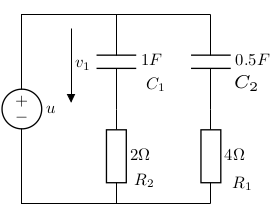
\includegraphics[width=0.4\textwidth]{lab3/rys1}
                \caption{}
                \label{fig:1}
            \end{figure}
            \begin{itemize}
                \item Układ z rysunku \ref{fig:1} nie jest sterowalny ponieważ $R_1C_1=R_2C_2$.
                \begin{figure}[H]
                    \centering
                    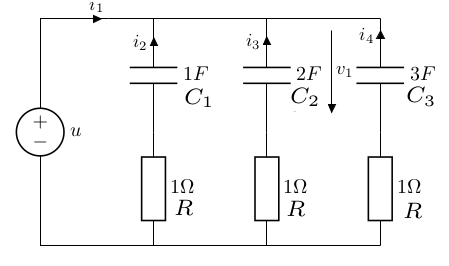
\includegraphics[width=0.4\textwidth]{lab3/rys2}
                    \caption{}
                    \label{fig:2}
                \end{figure}
                \item Układ z rysunku \ref{fig:2} jest sterowalny.
                \begin{figure}[H]
                    \centering
                    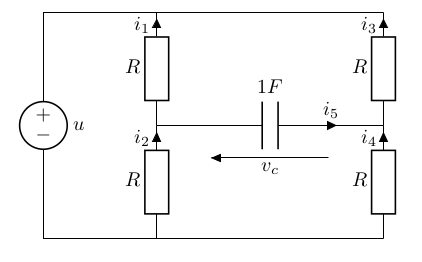
\includegraphics[width=0.4\textwidth]{lab3/rys3}
                    \caption{}
                    \label{fig:3}
                \end{figure}
                \item Układ z rysunku \ref{fig:3} nie jest sterowalny, ponieważ wszystkie rezystancje są sobie równe.\\
                Dlatego nie możemy sterować stanem kondensatora.
                \begin{figure}[H]
                    \centering
                    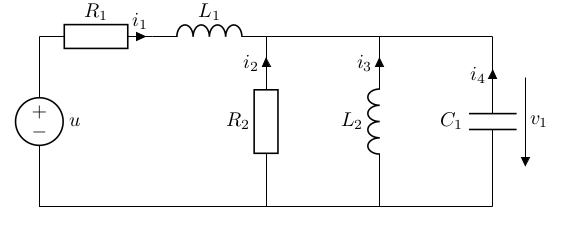
\includegraphics[width=0.4\textwidth]{lab3/rys4}
                    \caption{}
                    \label{fig:4}
                \end{figure}
                \item Układ z rysunku \ref{fig:4} jest sterowaly.
            \end{itemize}
            \textbf{\newline Jakie cechy układu pozwalają wnioskować o jego sterowalności?}\\
            Jeśli dla dowolnych warunków początkowych oraz dowolnej
            wybranej konfiguracji końcowej znaleźć można sygnał wejściowy pozwalający prze-
            prowadzić układ ze stanu pozcątkowego do stanu końcowego w skończonym czasie.\\\\
            \textbf{Jaki charakter będą miały odpowiedzi układów sterowalnych, a jaki niesterowalnych?}\\
            Charakter odpowiedzi będzie niezależny od zadanego sygnału sterującego.

        \itemcl[\begin{itemize}
            \item Rysunek \ref{fig:1}
                \[i_c=C\frac{d}{dt}u_c\]
                \[u=i_cR+v_c\]
                \[u=RC\frac{d}{dt}v_c+v_c\]
                \[RC\frac{d}{dt}v_c=u-v_c\]
                \[\frac{d}{dt}v_c=-\frac{1}{RC}v_c+\frac{1}{RC}u\]
                \[\begin{cases}
                    x_1=v_{C_1}\\
                    x_2=v_{C_2}\\
                    y_1=x_1\\
                    y_2=x_2
                \end{cases}\]
                \[\begin{cases}
                    \dot{x_1}=-\frac{1}{R_1C_1}x_1+\frac{1}{R_1C_1}u\\
                    \dot{x_2}=-\frac{1}{R_2C_2}x_2+\frac{1}{R_2C_2}u
                \end{cases}\]
                \[\dot{x}=
                \begin{bmatrix}
                    -\frac{1}{R_1C_1}& 0\\
                    0& -\frac{1}{R_2C_2}
                \end{bmatrix}x+
                \begin{bmatrix}
                    \frac{1}{R_1C_1}\\
                    \frac{1}{R_2C_2}
                \end{bmatrix}u\]
                \[y=
                \begin{bmatrix}
                    1&0
                \end{bmatrix}x+
                \begin{bmatrix}
                    0
                \end{bmatrix}u\]

            \item Rysunek \ref{fig:2}
                \[\dot{x}=
                \begin{bmatrix}
                    -\frac{1}{RC_1}& 0& 0\\
                    0& -\frac{1}{RC_2}& 0\\
                    0& 0& -\frac{1}{RC_3}
                \end{bmatrix}x+
                \begin{bmatrix}
                    \frac{1}{RC_1}\\
                    \frac{1}{RC_2}\\
                    \frac{1}{RC_3}
                \end{bmatrix}u\]
                \[y=
                \begin{bmatrix}
                    0&0&1
                \end{bmatrix}x+
                \begin{bmatrix}
                    0
                \end{bmatrix}u\]

            \item Rysunek \ref{fig:3}
                \[i_3+i_4=i_1+i_2\]
                \[i_1R=v_c+i_3R,\text{ }i_2R=-v_c+i_4\]
                \[i_5=C\frac{d}{dt}v_c=i_2-i_1=i_3-i_4\]
                \[i_1=\frac{1}{R}v_c+i_2,\text{ }i_2=-\frac{1}{R}v_c+i_4\]
                \[i_5=-\frac{1}{R}v_c-\frac{1}{R}v_c+i_4+i_3\]
                \[i_5=-\frac{1}{R}v_c-i_5\]
                \[2C\frac{d}{dt}v_c=-\frac{1}{R}v_c-\frac{1}{R}v_c\]
                \[\frac{d}{dt}v_c=-\frac{1}{CR}v_c\]
                \[\begin{cases}
                    x=v_c\\
                    \dot{x}=-\frac{1}{CR}x\\
                    y=x
                \end{cases}\]
                \[\dot{x}=
                \begin{bmatrix}
                    -\frac{1}{CR}
                \end{bmatrix}x+
                \begin{bmatrix}
                    0
                \end{bmatrix}u\]
                \[y=
                \begin{bmatrix}
                    1
                \end{bmatrix}x+
                \begin{bmatrix}
                    0
                \end{bmatrix}u\]

            \item Rysunek \ref{fig:4}
                \[v_L=L\frac{d}{dt}i_L\]
                \[v_1=L_2\frac{d}{dt}i_3\]
                \[v_1=i_2R_2\]
                \[v_1=-u+i_1R_1+L_1\frac{d}{dt}i_1\]
                \[i_4=-i_1-i_2-i_3\]
                \[C_1\frac{d}{dt}v_1=-i_1-\frac{1}{R_2}v_1-i_3\]
                \[\begin{cases}
                    x_1=i_1\\
                    x_2=i_2\\
                    x_3=v_1
                \end{cases}\]
                \[\dot{x}=\begin{bmatrix}
                    -\frac{R_1}{L_1}& 0& \frac{1}{L_1}\\
                    0& 0& \frac{1}{L_2}\\
                    -\frac{1}{C_1}& -\frac{1}{C_1}& -\frac{1}{C_1R_2}
                \end{bmatrix}x+
                \begin{bmatrix}
                    \frac{1}{L_1}\\0\\0
                \end{bmatrix}u\]
                \[y=\begin{bmatrix}
                    0&0&1
                \end{bmatrix}x+
                \begin{bmatrix}
                    0
                \end{bmatrix}u\]
                
            \end{itemize}
            ]{Wyznaczyć modele układów z Rys. 1-4. Przedstawić modele w przestrzeni zmiennych
            stanu.}{lab3.py}{1}{88}
            \textbf{Czy możliwe jest uzyskanie innych modeli w przestrzeni zmiennych stanu?}\\
            Jest możliwe uzyskanie innych modeli w przestrzeni zmiennych stanu.

        \itemcl[]{Wyznaczyć macierze Kalmana i formalnie zbadać sterowalność układów (wykorzystać na
            przykład \emph{numpy.linalg.matrix\_rank}).}{lab3.py}{91}{107}
            \outputTxt{snippets/lab3/zad1_3.txt}

        \itemcl[]{Zaimplementować przedstawione układy i zbadać ich odpowiedzi na wybrane wymuszenia
            (np. wymuszenie skokowe, wymuszenie sinusoidalne, wykorzystać na przykład
            \emph{scipy.signal.lsim} lub \emph{scipy.signal.lsim2}).}{lab3.py}{110}{137}
            \outputImg{0.7}{lab3/zad1_4_1}
            \outputImg{0.7}{lab3/zad1_4_2}
            \outputImg{0.7}{lab3/zad1_4_3}
            \outputImg{0.7}{lab3/zad1_4_4}
            \textbf{Czy uzyskane przebiegi potwierdzają wcześniejsze przypuszczenia?}\\
            Odpowiedzi dla układu z rysunku \ref{fig:1} nie potwierdzają wcześniejszych przypuszczeń.\\\\
            \textbf{Jakie są różnice między różnymi funkcjami symulującymi układy w Pythonie?}\\
            Funkcje \emph{scipy.signal.lsim} i \emph{scipy.signal.lsim2} dla układów liniowych,
            z tym że \emph{lsim2} nie wymaga podawania wektorów czasu i wymuszenia. W przypadku
            nie podania wektora wymuszenia, domyślne wymuszenie to zero. W przypadku nie podania
            wektora czasu, domyśly wektor czasu to \emph{numpy.linspace(0, 10, 101)}. Obie te
            funkcje przyjmują układ liniowy w postaci klasy \emph{lti} lub interpretacji układu
            w postaci \emph{tuple} 2,3, lub 4 elementowej.\\
            Funkcja \emph{scipy.integrate.solve\_ivp} różni się od powyższych funkcji głównie tym,
            że reprezentacja układu podawana jest w postaci ręcznie zdefiniowanej funkcji różniczkowej.\\
            Funkcje \emph{scipy.signal.step} oraz \emph{scipy.signal.impulse} przyjmują układ
            liniowy w postaci klasy \emph{lti} lub interpretacji układu w postaci
            \emph{tuple} 2,3, lub 4 elementowej. Obliczają kolejno odpowiedź skokową i impulsową układu.
            Jeżeli wektor czasu nie zostanie podany, jest on automatycznie wyliczany.
    
        \itemcl[]{Dla układów sterowalnych z poprzednich zadań wyznaczyć postać sterowalną równań
            dynamiki. Do wykonania obliczeń wykorzystać funkcjonalności Pythona.}{lab3.py}{140}{154}
            \outputTxt{snippets/lab3/zad2_1.txt}
            \textbf{Czy dla układów niesterowalnych można wyznaczyć postać normalną regulatorową
            dynamiki? Dlaczego?}\\
            Można wyznaczyć postać normalną regulatorową dla układów niesterowalnych, jeżeli stopień
            licznika jest mniejszy niż stopień mianownika w transmitancji. Ponieważ jest to jedynie
            inna reprezentacja tego samego układu.

        \itemcl[]{Dla wybranego przypadku przeprowadzić symulację obiektu dla obu reprezentacji (tj.
        wyznaczonej samodzielnie w zadaniu 1.2 oraz normalnej regulatorowej).}{lab3.py}{157}{171}
        \outputImg{1}{lab3/zad2_2}
        \textbf{Czy obie reprezentacje są równoważne?}\\
        Tak\\\\
        \textbf{Czy przebiegi dla obu reprezentacji są jednakowe? Dlaczego? Jakie będzie miało
        to znaczenie przy projektowaniu układu regulacji w oparciu o postać sterowalną?}\\
        Przebiegi nie są jednakowe dla obu reprezentacji. Jest to związane z tym że inaczej
        zostały przyjęte równania stanów przejściowych. Jednak wyjście układu jest jednakowe
        dla obu reprezentacji. Przy projektowaniu układu regulacji w oparciu o postać sterowalną
        mamy tą zaletę że każdy stan jest pochodną stanu poprzedniego, a wyjście jest sumą stanów
        pośrednich pomnożonych przez współczynniki, co sprowadza dostrajanie układu
        do regulacji współczynników.

    \end{enumerate}

\end{document}